\chapter{Mengenlehre}
\index{Mengenlehre}
%
Die Mengenlehre ist ein Teilgebiet der Mathematik und beschäftigt sich mit Sammlungen von unterscheidbaren Objekten. Da in der Informatik das Konzept der Mengen oft wiederverwendet wird, sei eine oberflächliche, aber präzise Betrachtungsweise gegeben.

Eine \emph{Menge} (engl. Set) ist
\begin{itemize}
 \item ungeordnet
 \item jedes Element unterscheidet sich von anderen Elementen in dieser Menge und kommt daher nur einmal vor
 \item besitzt eine beliebige Anzahl von Elementen
\end{itemize}
%
Die \emph{leere Menge} wird mit $\diameter$ oder $\{\}$ bezeichnet. Die Anzahl der Elemente einer Menge nennt man auch \emph{Kardinalität einer Menge}. Zur Notation der Kardinalität werden vertikale Balken um die Menge verwendet. So haben wir etwa in Abschnitt~\ref{sec:bits_numeric_systems_10} von $|\text{Alphabet}_{\text{dec}}|$ gesprochen, womit die Anzahl der Elemente der Menge Alphabet im Dezimalsystem gemeint ist. Die Definition der Mengen erlaubt sowohl endliche als auch unendliche Mengen\footnote{Die Diskussion um die Definition eines Unendlichkeitsbegriffs und der Abgrenzung zum Begriff ,,endlich abzählbar`` entstammt direkt der Mengenlehre. Als guter Einstieg in die Thematik dient der Satz von Cantor.}. Mengen werden wie Matrizen per Konvention mit einem Großbuchstaben bezeichnet.
%
\[
   A = \{1, 2, 3, 4\}
\] \[
   B = \{\}
\]

\section{Mengennotation}
\index{Mengennotation}
%
Wir stellen fest dass geschwungene Klammern genutzt werden, um Mengen zu definieren. Innerhalb dieser Klammern sind die Elemente dieser Menge kommagetrennt aufgelistet. Diese Notation reicht jedoch nicht immer aus, um beliebige Mengen zu spezifizieren.

Die Mengennotation (engl. ,,set-builder notation``, ,,set comprehension``) erlaubt es uns zwischen den geschwungenen Klammern einen vertikalen Balken (oder einen Doppelpunkt) zu verwenden. Wenn die Kriterien auf der rechten Seite des Balkens erfüllt sind, wird das Element auf der linken Seite aufgenommen. Domänenkriterien (zB. $t \in \mathbb{N}$) dürfen jedoch auch auf der linken Seite genannt werden, wenn sie sich nur auf das auszuwählende Element beziehen. Auf diesem Weg können wir auch unendliche Mengen abbilden.

\[
    C = \{x^2 | x \in \mathbb{N}\}
\] \[
    D = \{x | x^2 \mod{p} = 0, x \in \mathbb{N}\}
\] \[
    E = \{x \in \mathbb{N} | x^2 \mod{p} = 0\}
\]

\section{Eindeutigkeit und Abgrenzungen zu ähnlichen Begriffen}
\index{Liste}
\index{Sequenz}
\index{Tupel}
\index{Menge}
%
Entsprechend der genannten Definition darf jedes Element genau nur einmal vorkommen. Obwohl diese Definition oft respektiert wird, wird sie im Allgemeinen inkonsistent verwendet. So wird auch die Sequenz ($\{1, 2, 3, 2\}$) als Menge bezeichnet. Die Frage ist, wie sich die Begriffe Liste, Sequenz, Tupel und Menge voneinander abgrenzen. Wir möchten hier einen abstrakten Überblick geben, da die Unterschiede zur Definition von Datenstrukturen in der Programmierung relevant sind.
%
\begin{description}
 \item[Liste] Eine Liste ist eine geordnete Sammlung von beliebig vielen Elementen.
 \item[Sequenz] Eine Sequenz ist eine geordnete Sammlung von beliebig vielen Elementen,
                die meisten auf eine endliche Größe beschränkt sind.
 \item[Tupel] Eine geordnete Sammlung von homogenen Elementen endlicher Anzahl.
 \item[Menge] Ungeordnete Sammlung von unterschiedlichen Objekten.
\end{description}

Alle Begriffe erlauben grundsätzlich Verschachtelungen (zB Liste in Liste),
werden jedoch oft nur eindimensional verwendet.

\section{Elementare Mengenoperationen}
%
\subsection{Vereinigung}
\index{Vereinigung (Mengenoperation)}
%
Gegeben seien 2 Mengen $A$ und $B$. Die \emph{Vereinigung} (engl. ,,union``) der Mengen
$A$ und $B$ ist die Menge der Elemente, die in $A$ \emph{oder} $B$ vorkommen.
Dies bedeutet wir können den logischen Operator Oder verwenden, um aufgenommene
bzw. abgelehnte Elemente der Vereinigungsmenge zu spezifizieren. Hier ergibt
sich eine Schnittstelle zwischen Logik und Mengenlehre:
%
\[
    A \cup B = \{x \,|\, (x \in A) \lor (x \in B)\}
\]
%
\begin{figure}[p]
 \begin{center}
  \includegraphics{img/union.pdf}
  \caption{Illustration der Vereinigungsmenge (rote Menge $A$, blaue Menge $B$,
        Vereinigungsmenge $A \cup B$ als violette Umrandung)}
  \label{fig:union}
 \end{center}
\end{figure}

\subsection{Durchschnitt oder Schnittmenge}
\index{Durchschnitt (Mengenoperation)}
\index{Schnittmenge (Mengenoperation)}
%
Gegeben seien 2 Mengen $A$ und $B$. Der \emph{Durchschnitt} (engl. ,,intersection``)
der Menge $A$ und $B$ ist die Menge jener Elemente, die in $A$ \emph{und}
$B$ vorkommen:
\[
    A \cap B = \{x \,|\, (x \in A) \land (x \in B)\}
\]
%
\begin{figure}[p]
 \begin{center}
  \includegraphics{img/intersection.pdf}
  \caption{Illustration des Durchschnitts (rote Menge $A$, blaue Menge $B$,
        violetter Durchschnitt $A \cap B$)}
  \label{fig:union}
 \end{center}
\end{figure}

\subsection{Komplement oder Differenz}
\index{Komplement, relativ (Mengenoperation)}
%
Gegeben seien 2 Mengen $A$ und $B$. Das \emph{relative Komplement} der Menge $A$ und $B$
ist die Menge jener Elemente, die in $A$, aber nicht in $B$, vorkommen.
\[
    A \setminus B = \{x \,|\, (x \in A) \land (x \notin B)\}
\]
%
\begin{figure}[p]
 \begin{center}
  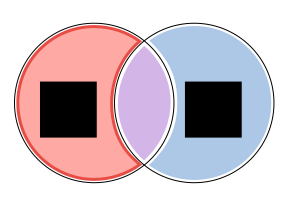
\includegraphics{img/complement.pdf}
  \caption{Illustration des Komplements (rote Menge $A$, blaue Menge $B$,
        rotes Komplements $A \setminus B$)}
  \label{fig:complement}
 \end{center}
\end{figure}

\subsection{Teilmenge}
\index{Teilmenge (Mengenrelation)}
%
Die Teilmenge beschreibt eine Relation und erzeugt keine neue Menge.
Ihr Ergebnis ist also eine ,,Ja`` oder ,,Nein`` Antwort.
Eine Menge ist eine Teilmenge einer anderen Menge genau dann wenn alle
Elemente der Teilmenge in ihr enthalten sind. $A$ ist eine
Teilmenge von $B$ genau dann wenn $A \subseteq B$:
\[
    A \subseteq B \text{ iff } \forall x \in A, x \in B
\]

Wir grenzen hierbei ,,echte Teilmengen`` ($A \neq B $, Operator $\subset$)
von ,,Teilmengen`` ($A = B \lor A \subset B$, Operator $\subseteq$) ab.

\subsection{Mitgliedschaft}
\index{Mitgliedschaft (Mengenrelation)}
%
Eine weitere Relation ist die Mitgliedschaft.
Für jede Menge kann getestet werden, ob ein Element enthalten ist. Als Beispiel
sei die Menge $C = \{x^2 | x \in \mathbb{N}\}$ gegeben. Darin sind etwa die Elemente
$1, 4$ und $81$ enthalten. Die Frage der Mitgliedschaft lautet: $x \in C$ für
ein bestimmtes $x$?
\[
  4 \in C  \qquad  42 \notin C  \qquad  441 \in C
\]

\section{Darstellung von Mengen}
\index{Venn-Diagramm}
%
Möchte man Mengen und deren Relationen darstellen, bieten sich Venn-Diagramme an,
die eine intuitive Übersicht bieten. In Darstellung~\ref{fig:venn_diagram} können
wir auch ein Beispiel des Inklusion-Exklusion Prinzips sehen. Dieses besagt, dass
wir für die Beschreibung der Kardinalität von A, B \emph{und} C die einzelnen Kardinalitäten
der Mengen A, B und C betrachten müssen, die paarweisen Schnittmenge zu exkludieren
sind und anschließend die Schnittmenge aller drei Mengen wieder zu inkludieren ist.
Formal:
\[
    |A \cup B \cup C| = |A| + |B| + |C| - |A \cap B| - |A \cap C|
        - |B \cap C| + |A \cap B \cap C|
\]
%
\begin{figure}[p]
 \begin{center}
  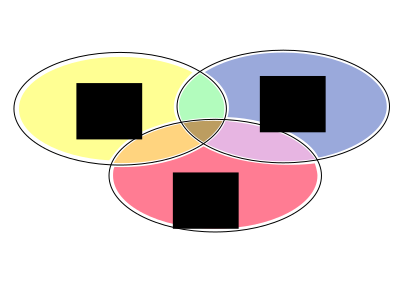
\includegraphics{img/venn_diagram_example.pdf}
  \caption{Venn Diagramm Beispiel}
  \label{fig:venn_diagram}
 \end{center}
\end{figure}

